\documentclass[a4paper]{article}

\usepackage[T1]{fontenc}
\usepackage[utf8x]{inputenc}

\usepackage[a4paper]{geometry}
\geometry{verbose,tmargin=3cm,bmargin=3cm,lmargin=2cm,rmargin=2cm,headheight=2cm,headsep=1cm,footskip=2cm}


\usepackage{fancyhdr}
\usepackage{enumerate}
\usepackage{adjustbox}
\pagestyle{fancy}
\setlength{\parskip}{\medskipamount}
\setlength{\parindent}{0pt}
\usepackage{graphicx}
\usepackage{listings}

\makeatletter

\usepackage{subcaption}
\usepackage{varwidth}
\usepackage{float} 
\usepackage{color}
\usepackage{lastpage}
\usepackage{indentfirst}

\lhead[lh-even]{Edgar Vedvik\\edgarmv}
\chead[ch-even]{TDT4173 Maskinlæring og case-basert resonnering\\Assignment 1}
\rhead[rh-even]{\today}

\lfoot[lf-even]{}
\cfoot[cf-even]{Page \thepage{} of \pageref{LastPage}}
\rfoot[rf-even]{}

\date{}
\makeatother
\usepackage[english]{babel}

\begin{document}
\thispagestyle{fancy}

\section{Theory}
\begin{enumerate}
    \item
        Concept learning is the problem of searching through a predefined space
        of potential hypotheses for the hypothesis that best fits the training
        examples.
    \item
        Function approximation is the task of selecting a function that
        approximates the target function. This is needed because finding a the
        target function could be very difficult, or the target function could
        be unknown.
    \item
        Inductive bias is the assumptions we make about the target concept, and
        allows us to generalize beyond the training examples the agent is
        given. The candidate elimination algorithm has the inductive bias of
        assuming the target concept is in the given hypothesis space, whereas
        decision tree learning has an inductive bias of preferring shorter trees
        over large trees and a preference for placing attributes with higher
        information gain closer to the top of the tree.
    \item
        Overfitting refers to a hypothesis or model that models the training
        data best, but performs worse than some other hypothesis against the
        entire distribution of instances. This can happen when there is noise
        in the data or there are too few training examples. Underfitting refers
        to a hypothesis that performs poorly on both training data and new
        data.

        A validation set is one part of the available training data. Some parts
        of the training data is kept for validation and not used for learning.
        The remaining training set is used to form the learned hypothesis and
        then the validation set is used to evaluate the accuracy of the
        hypothesis, and to evaluate the effect of pruning the tree.

        When splitting the validation set from the training set the hypothesis
        tends to be reflected by the way the data was divided. Cross validation
        is therefore used to make sure there is an equal chance for each
        example to appear in either set, so that the learning hypothesis does
        not completely match an example from the validation set.
    \item
        The candidate elimination algorithm begins with the version space of
        all hypotheses. As the algorithm learns it will contain all hypotheses
        that are consistent with an observed sequence of training examples. The
        version space is compactly stored as all possible hypotheses between
        two boundaries: the general boundary(G) and the specific boundary(S).
        At the beginning G is initialized to $\{<?,?,?,?>\}$ and S is
        initialized to $\{<\emptyset,\emptyset,\emptyset,\emptyset>\}$.

        \begin{table}[ht]
            \begin{center}
                \begin{tabular}{|c|c|c|c|c|}
                \hline
                \textbf{Sex} & \textbf{Problem Area} & \textbf{Activity Level} & \textbf{Sleep Quality} & \textbf{Treatment Successful}\\\hline
                Female & Back     & Medium & Medium & Yes\\\hline
                Female & Neck     & Medium & High   & Yes\\\hline
                Female & Shoulder & Low    & Low    & No\\\hline
                Male   & Neck     & High   & Medium & Yes\\\hline
                Male   & Back     & Medium & Low    & Yes\\\hline
                \end{tabular}
                \caption{Training data}
            \end{center}
        \end{table}

        The first training example is a positive one, and the algorithm must
        therefore check if the specific boundary covers the example. The
        updated boundaries can be seen in the first row of table
        \ref{tab:candidate-results}.  The second example further specializes S,
        making \textit{problem area} and \textit{sleep quality} more general.
        The third example is negative, and we must therefore make G less
        general so that it does not contain this example.  There are several
        hypotheses that would make G classify the new example as negative.
        However, only one is consistent with the S boundary. 

        When the fourth example is given, the specific boundary becomes so
        general that it contains every hypothesis. Since our general boundary
        hypothesis is inconsistent with this training example, we have to
        remove it, leaving us with no general boundary. This could mean there
        is an error in the dataset, or we do not have all the variables for
        correctly determining if the treatment was successful. After this
        example the algorithm should stop. 

        \begin{table}[ht]
            \begin{center}
            \begin{tabular}{|c|c|c|}
                \hline
                \# & S & G\\\hline
                0 & $\{<\emptyset, \emptyset, \emptyset, \emptyset>\}$ & $\{<?, ?, ?, ?>\}$\\\hline
                1 & $\{<Female, Back, Medium, Medium>\}$ & $\{<?, ?, ?, ?>\}$\\\hline
                2 & $\{<Female, ?, Medium, ?>\}$ & $\{<?, ?, ?, ?>\}$\\\hline
                3 & $\{<Female, ?, Medium, ?>\}$ & $\{<?, ?, Medium, ?>\}$\\\hline
                4 & $\{< ?, ?, ?, ?>\}$ & $\{\}$\\\hline
            \end{tabular}
            \caption{Results of candidate elimination on the physiotherapy questionnaire}
            \label{tab:candidate-results}
            \end{center}
        \end{table}

\end{enumerate}
\section{Programming}
\subsection*{Task 1: Linear Regression}
    \begin{enumerate}
        \item
            See the function \emph{ordinary\_least\_squares()} in \emph{linear\_regression.py}
        \item 
            After running the \emph{linear\_regression.py} file the following output is produced:
            \begin{lstlisting}[language=bash]
$ python3 linear_regression.py
Weights: [[0.24079271 0.48155686 0.0586439]]
Training data error: [0.01038685]
Test data error: [0.00952976]
            \end{lstlisting}
            Based on the relatively small error, we can say that the model generalizes well.

        \item
            After running the \emph{linear\_regression.py} file on the second dataset this
            output is produced:
            \begin{lstlisting}[language=bash]
$ python3 linear_regression.py
Weights: [[0.1955866  0.61288795]]
Training data error: [0.01375879]
Test data error: [0.01244246]
            \end{lstlisting}

            There is more error in this dataset than the previous, but it is still
            a good fit as can be seen in figure
            \ref{fig:linear-regression}.
            \begin{figure}[ht]
                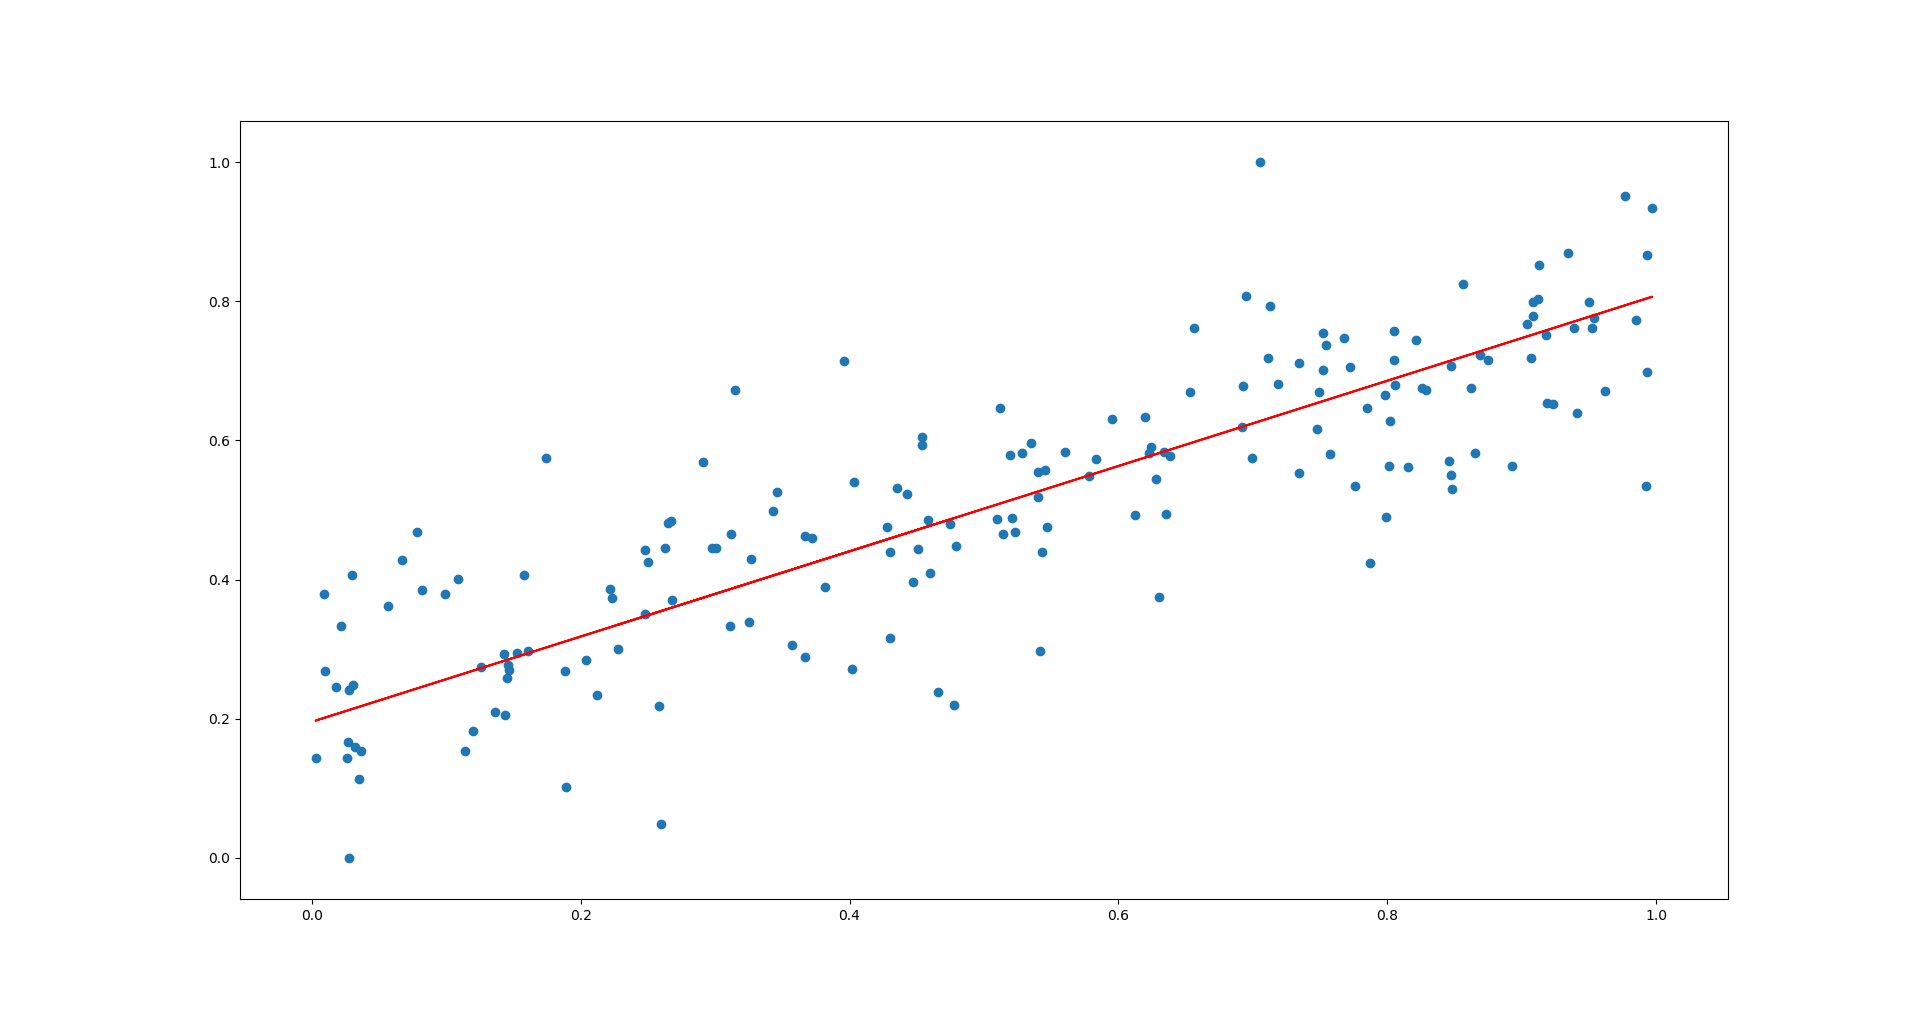
\includegraphics[width=\linewidth]{linear_regression.png}
                \caption{Linear regression of the test\_1d\_reg\_data.}
                \label{fig:linear-regression}
            \end{figure}
    \end{enumerate}
\subsection*{Task 2: Logistic Regression}
    \begin{enumerate}
        \item
            See \emph{logistical\_regression.py} for the implementations.

            The data is linearly separable because we can draw a straight line
            that separates the positive (1) examples from the negative examples
            (0).

            The cross entropy for both data sets, as they develop over 1000 iterations, can be
            seen in figure \ref{fig:cross-entropy}. The learning rate used was $\eta = 0.01$, and 
            the initial parameters $\textbf{w} = \{0, 0, 0\}$. After training was done the weights
            for the training set were $\textbf{w} = \{4.22448447, -12.27806252, 6.36330889\}$ and for
            the test set: $\textbf{w} = \{5.32779934, -10.79201844, 3.10085983\}$.

            \begin{figure}[ht]
                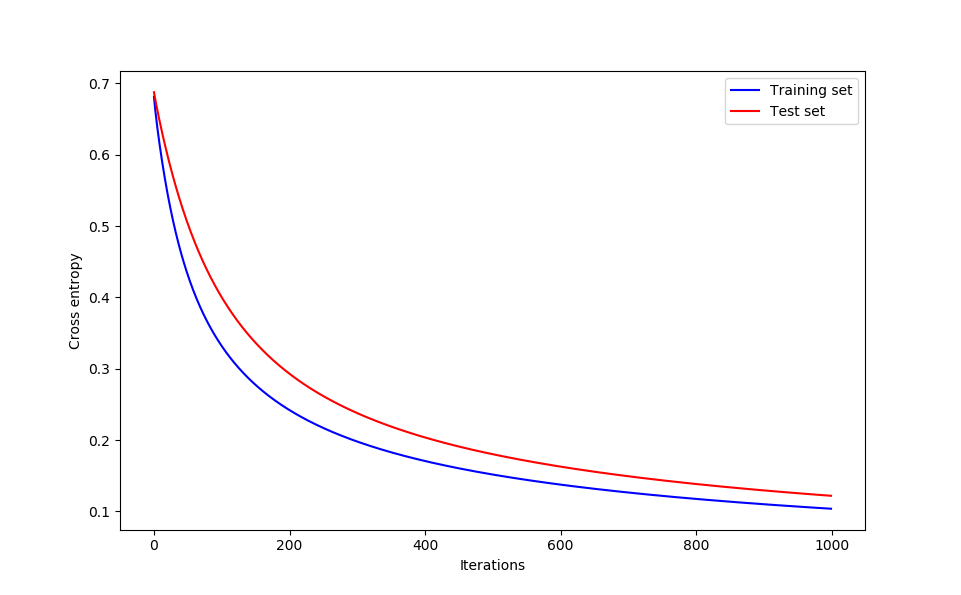
\includegraphics[width=\linewidth]{cross_entropy.png}
                \caption{Cross entropy error development for both the training and test data set}
                \label{fig:cross-entropy}
            \end{figure}

            Figure \ref{fig:logistical-regression} shows the decision boundary
            after running through the learning set. The blue dots represents
            inputs whose output should be 1, and red represents inputs whose
            output is 0. As we can see, the fit is very good with only one point
            that is on the wrong side of the decision line. This tells us it is
            generalizing well.

            \begin{figure}[h]
                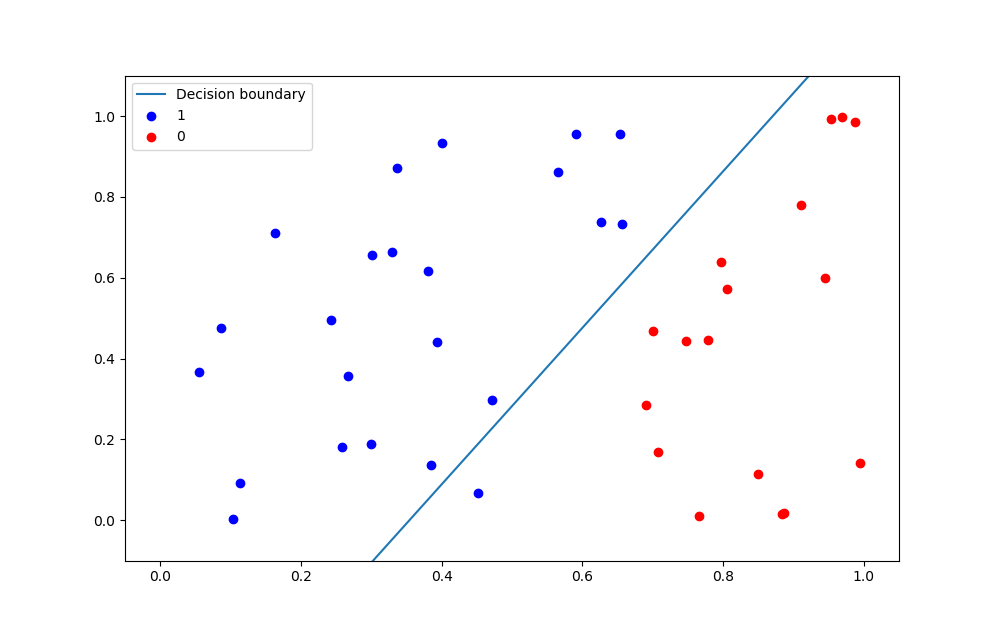
\includegraphics[width=\linewidth]{logistical_regression.png}
                \caption{Results of the test data after training.}
                \label{fig:logistical-regression}
            \end{figure}

        \item
            From figure \ref{fig:dataset2} we can see that there is no straight
            line that would be able to partition these points, so this data is
            not linearly separable. We also see the decision boundary calculated is
            not very good.

            \begin{figure}[h]
                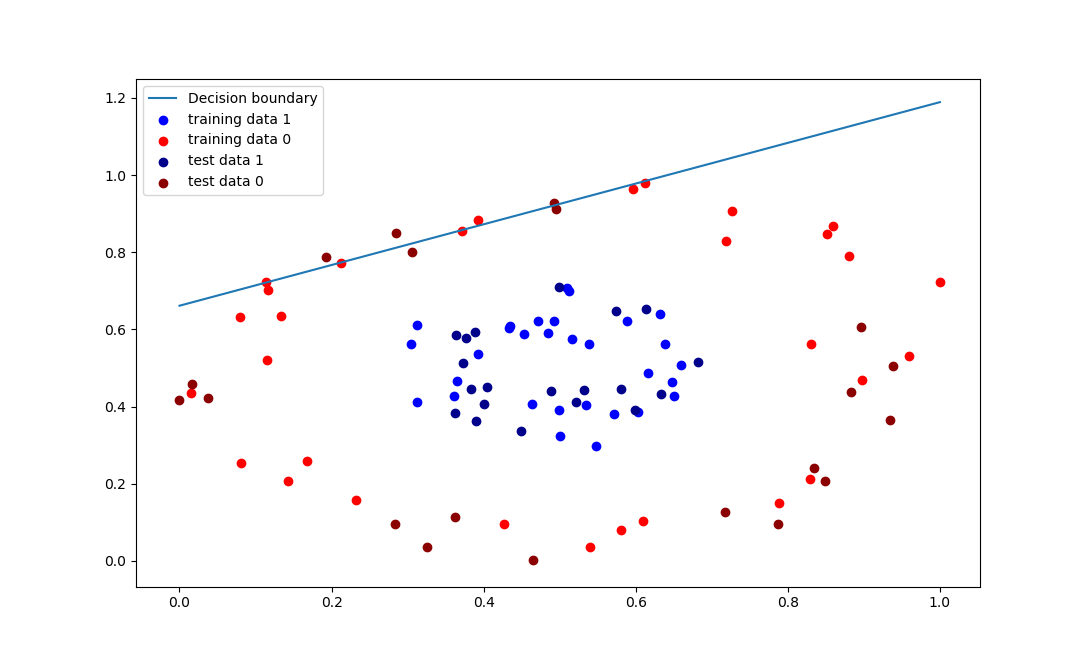
\includegraphics[width=\linewidth]{dataset2.png}
                \caption{Plot of second data sets with decision boundary.}
                \label{fig:dataset2}
            \end{figure}

            In order to correctly classify the dataset we have to create more
            features by multiplying together the features we already have so
            we go from $\textbf{w} = \{w_0, w_1, w_2\}$ to $\textbf{w} = \{w_0,
            w_1, w_2, w_1^2 w_2^2\}$.  This will allow us to create circular
            decision boundaries. The updated result was generated by
            \emph{regression\_1()} in \emph{logistical\_regression.py}, and the
            result can be seen in figure \ref{fig:dataset2-corrected}.

            \begin{figure}[h]
                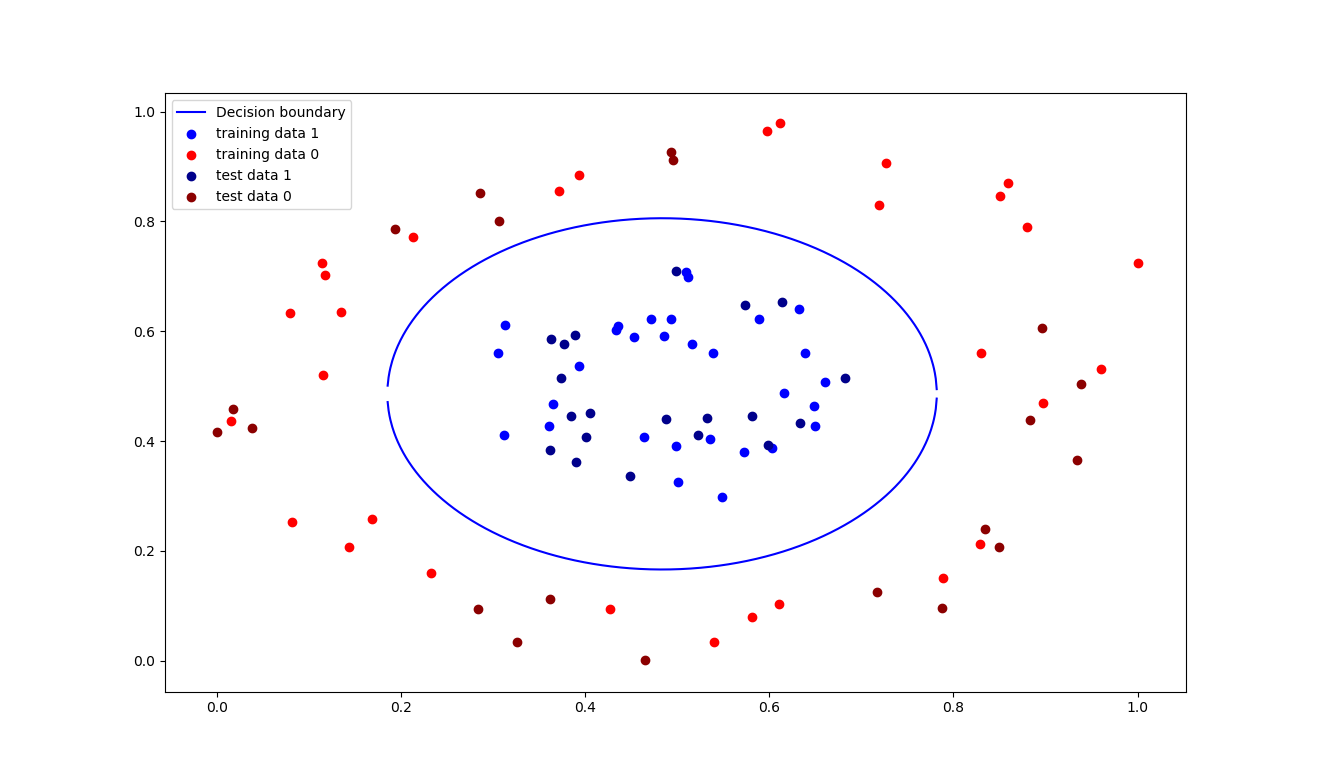
\includegraphics[width=\linewidth]{dataset2_corrected.png}
                \caption{An updated plot with the new decision boundary.}
                \label{fig:dataset2-corrected}
            \end{figure}

    \end{enumerate}
\end{document}
